\documentclass{beamer}
%
% Choose how your presentation looks.
%
% For more themes, color themes and font themes, see:
% http://deic.uab.es/~iblanes/beamer_gallery/index_by_theme.html
%
\mode<presentation>
{
  \usetheme{Madrid}      % or try Darmstadt, Madrid, Warsaw, ...
  \usecolortheme{beaver} % or try albatross, beaver, crane, ...
  \usefonttheme{serif}  % or try serif, structurebold, ...
  \setbeamertemplate{navigation symbols}{}
  \setbeamertemplate{caption}[numbered]
} 

\setbeamertemplate{caption}{\raggedright\insertcaption\par}

\usepackage[english]{babel}
\usepackage[utf8]{inputenc}
\usepackage[T1]{fontenc}
\usepackage{graphicx}
\usepackage{tikz}
\usetikzlibrary{shapes,snakes,arrows, chains, positioning, shapes.geometric, shapes.symbols,calc,shadows}

%tikzxommand
\def\centerarc[#1](#2)(#3:#4:#5)% Syntax: [draw options] (center) (initial angle:final angle:radius)
{ \draw[#1] ($(#2)+({#5*cos(#3)},{#5*sin(#3)})$) arc (#3:#4:#5); }


%commands
\newcommand{\C}{\mathbb{C}}
\newcommand{\R}{\mathbb{R}}
\newcommand{\CP}{\mathbb{CP}}
\newcommand{\mM}{\mathcal{M}}

\newcommand{\ddb}{\partial\overline{\partial}}
\DeclareMathOperator{\Met}{Met}
\DeclareMathOperator{\hot}{(h.o.t.)}

\newcommand{\mathcolorbox}[2]{\colorbox{#1}{$\displaystyle #2$}}

\title[]{Bubbling of K\"ahler-Einstein metrics with cone singularities: examples in dimensions \(1\) and \(2\)}
\author[Martin de Borbon]{Martin de Borbon (joint with Cristiano Spotti)}
\institute[Loughborough]{Seminar at Tsinghua University}
\date{5 December 2023}

\begin{document}

\begin{frame}
  \titlepage
\end{frame}

% Uncomment these lines for an automatically generated outline.
%\begin{frame}{Outline}
%  \tableofcontents
%\end{frame}

\section{Introduction}

\begin{frame}{Outline}
	\begin{itemize}
		\setlength{\itemsep}{\fill}
		\pause
		\item \(\dim_{\C} = 1\): Degeneration of polyhedral metrics on the \(2\)-sphere
		
		\pause
		\item \(\dim_{\C} = 2\): Model Calabi-Yau metrics on \(\C^2\) with cone singularities along a complex curve  
		
		\pause
		\item Conjectures
	\end{itemize}
\end{frame}

\section{dim 1}


\begin{frame}{The \(2\)-cone \(C(2\pi\beta)\)}
	\pause
	\begin{minipage}{0.15\textwidth}
		\begin{block}{}
			\(0<\beta<1\)
		\end{block}
	\end{minipage}
	\pause
	\begin{center}
	\scalebox{0.7}{	
	\begin{tikzpicture}
	%leftpart
	\filldraw[fill=green!20, draw=blue] (-2,0) -- (0,0) arc (0:220:2) -- (-2,0);
	\centerarc[thick](-2,0)(5:215:.7);
	\centerarc[<->,dashed,thick](-2,0)(225:355:1);
	%middle arrow
	\draw[->,dashed,thick] (1,1) to (3,1);
	%rightpart
	\filldraw[fill=green!20] (4,2) to[bend right] (7,2) -- (5.5,-1) -- cycle;
	\draw[dotted,thick] (4,2) to[bend left] (7,2);
	%nodes
	\node[scale=1.3](a) at (-2,1.1){\(2\pi\beta\)};
	\node[scale=1.3](b) at (0,-.5){identify};
	%\node[fill=red!20,draw,rounded corners, scale=1.5](c) at (-4.5,2.5){\(0<\beta<1\)};
	\end{tikzpicture}
	}
	\end{center}

\begin{itemize}
	\pause
	\item In polar coordinates \(g_{\beta} = dr^2 + \beta^2 r^2 d\theta^2\)
	\pause
	\item \textbf{Fact:} the induced complex structure on \(\R^2 \setminus \{0\}\) is \(\C^*\)
	\pause
	\item Proof: set \(z = r^{1/\beta}e^{i\theta}\) then \(g_{\beta}=|z|^{2\beta-2}|dz|^2\)
\end{itemize}
\end{frame}



\begin{frame}{Constant curvature surfaces with cone singularities}
	%\pause	
	\pause
	\begin{columns}
		\begin{column}{.38\textwidth}
			\[
			\begin{cases}
			dr^2 + \beta^2\sin^2 r d\theta^2  \\
			dr^2 + \beta^2 r^2 d\theta^2 \\
			dr^2 + \beta^2 \sinh^2r d\theta^2 
			\end{cases}
			\]
		\end{column}
	\pause	
		\begin{column}{.58\textwidth}
			\begin{figure}[t]
				\centering
				\scalebox{.7}{
					\begin{tikzpicture}
					\filldraw[fill=green!40, draw=black] (-1,2) -- (0,0) -- (1,2) to[bend left] (-1,2);
					\draw[dashed] (-1,2) to[bend left] (1,2);
					
					\filldraw[fill=green!40, draw=black] (-4,2) to[bend right] (-3,0) to[bend right] (-2,2) to[bend left] (-4,2);
					\draw[dashed] (-4,2) to[bend left] (-2,2);
					
					\filldraw[fill=green!40, draw=black] (2,2) to[bend left] (3,0) to[bend left] (4,2) to[bend left] (2,2);
					\draw[dashed] (2,2) to[bend left] (4,2);
					
					%\node[scale=1.4] at (-3,-.4) {\(K=1\)};
					%\node[scale=1.4] at (0,-.4) {\(K=0\)};
					%\node[scale=1.4] at (3,-.4) {\(K=-1\)};
					
					\node[] at (-3,2.6) {\((2\pi\beta)\sin r\)};
					\node[] at (0,2.6) {\((2\pi\beta)r\)};
					\node[] at (3,2.6) {\((2\pi\beta)\sinh r\)};
					
					\node[] at (-4.1,1) {\(r\)};
					\node[] at (-.8,1) {\(r\)};
					\node[] at (2.6,1) {\(r\)};
					\end{tikzpicture}	
				}
			\end{figure}
		\end{column}
	\end{columns}
	
\begin{columns}
	\pause
	\begin{column}{.48\textwidth}
		\begin{figure}
			\scalebox{.7}{
				\begin{tikzpicture}
				\filldraw[fill=yellow!70, draw=black] (-1,-2) to[bend right] (1,-2) to[bend right] (0,0) to[bend right] (-1,-2);
				
				\draw (-.4, -.35) to[bend right] (.4,-.35);
				\draw[dashed] (.4,-.35) to[bend right] (-.4,-.35);
				
				\draw (-1, -1.5) to[bend right] (-.6, -2.2);
				\draw[dashed] (-1, -1.5) to[bend left] (-.6, -2.2);
				
				\draw[dashed] (1, -1.5) to[bend right] (.6, -2.2);
				\draw (1, -1.5) to[bend left] (.6, -2.2);
				
				\node[] at (0,-.7) {\(2\pi \beta\)};
				\end{tikzpicture}		
			}
			\caption{Double of spherical triangle.  Constant curvature \(1\) metric on the \(2\)-sphere with \(3\) cone points.}
		\end{figure}
	\end{column}
	\pause
	\begin{column}{.48\textwidth}
		\begin{itemize}
			\item Orbifolds: \(\beta = 1/k\) for \(k \geq 2\) integer
			\item Modular curve \(\mathbb{H}/PSL(2, \mathbb{Z})\). Hyperbolic metric with two cone points \(1/2, 1/3\)
		\end{itemize}
	\end{column}
\end{columns}
\end{frame}


\begin{frame}{Flat metrics on the \(2\)-sphere with cone points}
	\begin{itemize}
		\pause
		\item Surface of a polyhedron in \(\R^3\)
		\pause
		\item Double of a polygon in \(\R^2\)
	\end{itemize}

	\begin{columns}
	\pause	
	\begin{column}{.48\textwidth}
		\begin{figure}
			\scalebox{.5}{
				\begin{tikzpicture}
				\draw (0,0) -- (2,0) -- (2,2) -- (0,2) -- (0,0);
				\draw (2.7,.7) -- (2.7,2.7) -- (.7,2.7);
				\draw[dashed] (0.7,2.7) -- (0.7,0.7) -- (2.7,0.7);
				\draw[dashed] (0,0) -- (.7,.7);
				\draw (0,2) -- (.7,2.7);
				\draw (2,0) -- (2.7,.7);
				\draw (2,2) -- (2.7, 2.7);
				\end{tikzpicture}
			}
			\caption{Surface of a cube. Flat metric on \(S^2\) with \(8\) cone points of total angle \(2\pi\beta=3(\pi/2)\).}
		\end{figure}
	\end{column}	
	\pause
	\begin{column}{.48\textwidth}
		\begin{figure}
			\scalebox{.7}{
				\begin{tikzpicture}
				\draw (-1,0) -- (0,2) -- (1,0) -- cycle;
				\draw[dashed] (-.7, .6) to[bend left] (-.4, 0) to[bend left] (-.7, .6);
				\draw[dashed] (.7, .6) to[bend left] (.4, 0) to[bend left] (.7, .6);
				\draw[dashed] (-.3, 1.4) to[bend right] (.3, 1.4) to[bend right] (-.3, 1.4);
				\end{tikzpicture}		
			}
			\caption{Double of a triangle with interior angles \(\pi\beta_i\). Flat metric on \(S^2\) with \(3\) cone points of total angle \(2\pi\beta_i\)}
		\end{figure}
	\end{column}
\end{columns}
\pause
\begin{equation}\tag{Gauss-Bonnet}
	\mathcolorbox{green!40}{
		\sum_{i=1}^n (1-\beta_i) = 2
	}
\end{equation}

\begin{itemize}
	\pause
	\item Surface of a cube: \(8 \cdot (1-3/4) = 2\) 
	\pause
	\item Double of a triangle: \(3 - (\beta_1+\beta_2 + \beta_3) = 2\)
\end{itemize}

\end{frame}

\begin{frame}{Existence and uniqueness}
	\begin{itemize}
		\pause
		\item Fix \(\vec{\beta} = (\beta_1, \ldots, \beta_n)\) with \(\sum_{i=1}^{n}(1-\beta_i) = 2\)
		\pause
		\item \(\Met(\vec{\beta}) = \) flat metrics on \(S^2\) with \(n\) cone points \(x_i\) of total angle \(2\pi\beta_i\) modulo marked (orientation preserving) isometry and scale
		\pause
		\item \(\mM_{0,n} = \) configuration of \(n\) distinct marked points in \(\CP^1\) up to the action of M\"obius transformations \(PSL(2, \C)\)
	\end{itemize}

\pause
\begin{theorem}[Troyanov]
	The forgetful map \(F: \Met(\vec{\beta}) \to \mM_{0,n}\) is a bijection
\end{theorem}

\pause
Proof: If \(x_1, \ldots, x_n \in \C\) then
\[
\left(\prod_{i=1}^{n} |z-x_i|^{2\beta_i-2}\right) |dz|^2
\]
extends smoothly over \(\infty\) and defines a flat (K\"ahler) metric on \(\CP^1\) with cone angles \(2\pi\beta_i\) at the points \(x_i\)

\end{frame}

\begin{frame}{Collision of two cone points}
	
	\begin{figure}[h]
		\centering
		\begin{tikzpicture}	
		\fill[yellow!40] (5.5, 0) -- (8, 0) -- (8, 2) -- (6, 1) ;
		\draw[dashed] (4, 0) to (5.5,0);
		\draw[] (5.5, 0) to (8,0);
		\draw[dashed] (4, 0) to (6,1);
		\draw[] (6, 1) to (8, 2);
		\draw[red, thick] (5.5, 0) to (6,1);
		\centerarc[](5.5,0)(0:60:.3);
		\centerarc[](6,1)(-109:19:.3);
		\centerarc[](4,0)(0:28: .5);
		
		%labels
		\draw  (4, -0.3) node (asd) [scale=.9] {\(\pi \gamma\)};
		\draw  (5.5, -.3) node (asd) [scale=.9] {\(\pi \beta_1\)};
		\draw  (6.6, .8) node (asd) [scale=.9] {\(\pi \beta_2\)};
		\draw (5.5,.45) node (asd) [scale=.9] {$\epsilon$};
		%\draw  (4, 2) node (asd) [scale=.9] {$\gamma + (1-\beta_1) + (1-\beta_2) = 1$};
		
		
		\end{tikzpicture}
		\caption{\(\mathcolorbox{green!40}{\gamma + (1-\beta_1) + (1-\beta_2) = 1}\)}
	\end{figure}
\end{frame}

\begin{frame}{Model flat metrics on \(\C\) with cone points}
	\begin{columns}
		\begin{column}{.48\textwidth}
			\begin{itemize}
				\item \(\mathcolorbox{orange!30}{\sum_{i=1}^{p}(1-\beta_i)<1}\)
				\[
				g_F = \left(\prod_{i=1}^{p}|z-x_i|^{2\beta_i-2}\right)|dz|^2
				\]
				\item flat K\"ahler metric on \(\C\) with cone angles \(2\pi\beta_i\) at \(x_i\)
				\item isometric to the \(2\)-cone \(C(2\pi\gamma)\) outside a compact set 
				\[
				\mathcolorbox{green!40}{
				1 - \gamma = \sum_{i=1}^{p}(1-\beta_i)
				}
				\]
			\end{itemize}
		\end{column}
		\begin{column}{.48\textwidth}
			\begin{figure}
				\centering
				\scalebox{.5}{
					\begin{tikzpicture}
					\fill[yellow!40] (-5, 5) -- (-2,-1) -- (-1, 0) -- (0,-1) -- (1, 0) -- (2,-1) -- (5,5) to[bend right] (-5,5);
					\draw (-5, 5) -- (-2,-1) -- (-1, 0) -- (0,-1) -- (1, 0) -- (2,-1) -- (5,5);
					\draw[dashed] (-5,5) to[bend left] (5,5);
					\draw (-5,5) to[bend right] (5,5);
					\draw (-2.25, -.5) to[bend right] (-1.5,.-.5);
					\draw[dashed] (-2.25, -.5) to[bend left] (-1.5,.-.5);
					\draw (1.5, -.5) to[bend right] (2.25,.-.5);
					\draw[dashed] (1.5, -.5) to[bend left] (2.25,.-.5);
					\draw (-.5,-.5) to[bend right] (.5,-.5);
					\draw[dashed] (-.5,-.5) to[bend left] (.5,-.5);
					
					\node[scale=1.5] at (0,-1.3) {$2\pi\beta_i$};
					\node[scale=1.5] at (0,3.9) {$2\pi\gamma$};
					\end{tikzpicture}
				}
			\end{figure}
			\[
			\lim_{\lambda \to 0} \lambda \cdot g_F = C(2\pi\gamma)
			\]
		\end{column}
	\end{columns}
\end{frame}

\begin{frame}{Bubble trees}
	Consider a family of flat metrics \(g_t\) for which a cluster of cone points \(x_1(t), \ldots, x_p(t)\) collides to \(0\) as \(t \to 0\)
	\begin{itemize}
		\pause
		\item For \(f \in \mathcal{O}_{\C, 0}\) let \(\nu(f) = \) order of vanishing of \(f\) at \(0\)
		\pause
		\item For \(r \geq 0\) we have an equivalence relation \(f \sim_r g\) if \(\nu(f-g) \geq r\)
		\pause
		\item If \(S = \{x_1(t), \ldots, x_p(t)\} \subset \mathcal{O}_{\C, 0}\) is a finite set then the equivalence classes of \(\sim_r\) make a tree \(\mathcal{T}\) with root \(S\) and leaves \(\{x_i(t)\}\)
		\pause
		\item To every non-leaf vertex \(\mathbf{v} \in \mathcal{T}\) we associate a model flat metric \(B_{\mathbf{v}}\) on \(\C\). The number of cone points of \(B_{\mathbf{v}}\) is equal to the number of children of \(\mathbf{v}\)
		\pause
		\item  The cone angles are \(2\pi\gamma_{\mathbf{w}}\) with \(1-\gamma_{\mathbf{w}} = \sum_{i | x_i \in \mathbf{w}} (1-\beta_i)\) and the position of the cone points are \(x_{\mathbf{w}} = \lim_{t \to 0} t^{-k} x_i(t)\) where \(k\) is the smallest integer such that the elements of \(\mathbf{v}\) are \emph{not} \(\sim_k\) equivalent.  
	\end{itemize}
\end{frame}

\begin{frame}{Rescaled limits}
	\begin{itemize}
		\item Let \(s \in \mathcal{O}_{\C, 0}\) be a section
		\item For \(\alpha>0\) let \(h_{\alpha}\) be the pointed Gromov-Hausdorff limit 
		\[h_{\alpha} = \lim_{t \to 0} (|t|^{-2\alpha} \cdot g_t, s(t))\]
		\pause
		\item The section determines a path in the tree with vertices \(\mathbf{v}_1, \ldots, \mathbf{v}_{\ell}\)
		\item  \(0= \alpha_0 < \alpha_1 < \ldots < \alpha_{\ell}\) such that \(h_{\alpha} = C(2\pi \gamma_{\mathbf{v}_i})\) (with base point its vertex) if \(\alpha_{i-1} < \alpha < \alpha_i\) and \(h_{\alpha} = B_{\mathbf{v}_i}\) if \(\alpha=\alpha_i\) (with base point \(\lim_{t \to 0} t^{-k}s(t)\)).
	\end{itemize}
	
	\begin{figure}[h]
		\centering
		\begin{tikzpicture}
		\path (0,0) node(r) {$\{x_1, \ldots, x_4\}$} 
		(-2,-1) node(a) {$\{x_1, x_2, x_3\}$}
		(2,-1) node(b) {$\{x_4 = t^2\}$}
		(-4,-2) node(c) {$\{x_1 = t\}$}
		(-2,-2) node(d) {$\{x_2 = t - t^4\}$}
		(.5,-2) node(e) {$\{x_3 = t + t^4\}$};
		\draw[->, red, thick] (r) to (a);
		\draw[->] (r) to (b);
		\draw[->] (a) to (c);
		\draw[->, red, thick] (a) to (d);
		\draw[->] (a) to (e);
		\end{tikzpicture}
		\caption{$s(t) = t - t^4 + \text{(h.o.t.)}$ shown in red where \(\mathcal{T}\)}
		\label{fig:polytreepath}
	\end{figure}
	
\end{frame}

\begin{frame}{Moduli spaces}
	\begin{itemize}
		\setlength{\itemsep}{\fill}
		\item Thurston: complex hyperbolic cone metric on \(\overline{\Met}(\vec{\beta})\), divisors represent collision of pair of points
		\pause
		\item Deligne-Mumford-Knudsen compactification \(\overline{\mM}_{0,n}\), divisors correspond to partitions of \(\{1, \ldots, n\}\) into two disjoint sets, its points represent nodal curves with \(2\) irreducible components
		\pause
		\item Logarithmic resolution \(\overline{\mM}_{0,n} \to \overline{\Met}(\vec{\beta})\) (Koziarz-Nguyen), points in \(\overline{\mM}_{0,n}\) represent bubble trees
	\end{itemize}
\end{frame}

\section{dim 2}


\begin{frame}{K\"ahler-Einstein metrics with cone singularities}
	\begin{columns}
		\begin{column}{0.4\textwidth}
			\(D \subset X\) \emph{smooth} complex hypersurface and \(0<\beta<1\) 
		\end{column}
		\begin{column}{0.1\textwidth}
			\(\hspace{7mm} \longleftrightarrow\)
		\end{column}
		\begin{column}{0.4\textwidth}
			\begin{equation*}
			\mbox{\Large \(
				(X, (1-\beta)D) \)
			}
			\end{equation*}
		\end{column}
	\end{columns}
	
	\begin{center}
		\scalebox{0.7}{
			\begin{tikzpicture}
			\filldraw[yellow!40] plot [smooth cycle] coordinates {(-2,0) (1,3) (3,1) (2,-.5) (0,-2)};
			\draw (0,1) circle[radius=.7]; 
			\draw [blue, thick] plot [smooth, tension=.7] coordinates { (-1,0) (0,1) (1,1) (1.5,0) (2,-.3)};
			\draw[->, dashed] (.7,1.5) to[bend left] (8,1.5);
			\draw[blue, thick] (10,-2) to (10,3);
			
			%cones
			\draw[green,thick] (10,-.5) to (11,0);
			\draw[green,thick] (10,-0.5) to (11,-1);
			%\draw[green, thick, dashed] (9,-1) to[bend left] (9,0);
			%\draw[green, thick, dashed] (9,-1) to[bend right] (9,0);
			\draw[green, thick, dashed] (11,-1) to[bend left] (11,0);
			\draw[green, thick, dashed] (11,-1) to[bend right] (11,0);
			\draw[green,thick] (10,1.5) to (11,2);
			\draw[green,thick] (10,1.5) to (11,1);
			%\draw[green, thick, dashed] (9,1) to[bend left] (9,2);
			%\draw[green, thick, dashed] (9,1) to[bend right] (9,2);
			\draw[green, thick, dashed] (11,1) to[bend left] (11,2);
			\draw[green, thick, dashed] (11,1) to[bend right] (11,2);
			%\draw[green, thick] (-.4,1.3) .. controls (0,1) .. (.4,.6);
			%\draw[green, thick] (-.1,.55) .. controls (0,1) .. (0.1,1.45);	
			\draw[green,thick] (-.4,1.3) to (0,1);
			\draw[green,thick] (0.1,1.45) to (0,1);
			\draw[green, thick, dashed] (-.4,1.3) to[bend left] (0.1,1.45);
			\draw[green, thick, dashed] (-.4,1.3) to[bend right] (0.1,1.45);
			%\draw[green, thick, dashed] (.4,.6) to[bend left] (-.1,.55);
			%\draw[green, thick, dashed] (.4,.6) to[bend right] (-.1,.55);
			
			%nodes
			\node[scale=1.3](a) at (0,-1){\(X\)};
			\node[scale=1.3, blue](b) at (1.5,.8){\(D\)};
			\node[scale=1](c) at (11.6,1.5){\(2\pi\beta\)};
			\node[scale=1.3](a) at (12,3){\(C(2\pi\beta) \times \C^{n-1}\)};
			\end{tikzpicture}
		}
	\end{center}



\begin{itemize}
	\centering
	\item \(\mbox{Ric}(g_{KE}) = \lambda \cdot g_{KE}\) on \(X \setminus D\)
	\item \(g_{KE} \sim C(2\pi\beta) \times  \C^{n-1}\) near \(D\)
\end{itemize}


\end{frame}

\begin{frame}{Theory overview}
	\begin{itemize}
		\setlength{\itemsep}{\fill}
		\pause
		\item Donalson's interior Schauder estimate for the Laplace operator
		\pause
		\item Existence and regularity theory, polyhomogeneous expansion (Jeffress-Mazzeo-Rubinstein)
		\pause
		\item Chern-Weil formulas (Jian Song and Xiaowei Wang)
		\pause
		\item Algebraic structure on non-collapsed Gromov-Hausdorff limits (Chen-Donaldson-Sun)
	\end{itemize}
\end{frame}

\begin{frame}{Model Ricci-flat solutions}
\begin{columns}	
	\begin{column}{0.48\textwidth}
		\begin{figure}
			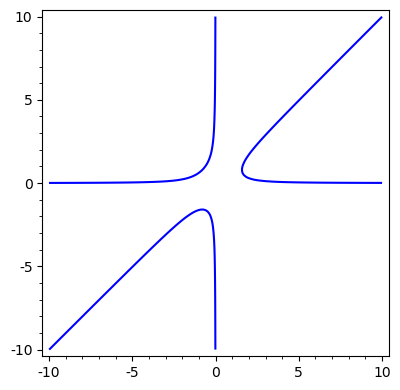
\includegraphics[width=0.8\textwidth,height=0.8\textheight,keepaspectratio]{cubic}
		\end{figure}
	\end{column}
	\begin{column}{0.48\textwidth}
		\begin{itemize}
			\item \(C=\{P=0\} \subset \C^2\) smooth with \(\mbox{deg}(P)\geq 2\)
			\item \emph{Different} asymptotic lines \\
			i.e. \emph{no} parabola
		\end{itemize}
	\begin{center}
		\begin{minipage}{0.4\textwidth}
			\begin{block}{}
				\(\frac{d-2}{d}<\beta<1\)
			\end{block}
		\end{minipage}
	\end{center}
	\end{column}
\end{columns}	
%\begin{equation*}
%C = \{P=0\}, \hspace{3mm} \mbox{deg}(P) = d\geq 2 .
%\end{equation*}
\pause
\begin{theorem}[de Borbon, 2017]
	\begin{enumerate}
		\item \(\omega_{RF}^2 = \Omega \wedge \bar{\Omega}\) with \(\Omega = P^{\beta-1} dz dw \) 
		\item \(\omega_{RF}\) is asymptotic to a polyhedral K\"ahler cone at infinity.
	\end{enumerate}
\end{theorem}
\end{frame}

\begin{frame}{Polyhedral K\"ahler cones}
	
	\begin{columns}
		\begin{column}{.38\textwidth}
			\begin{center}
				\(\bar{g} =\) constant curvature \(1\) metric on the \(3\)-sphere
			\end{center}		
		\end{column}
		\begin{column}{.68\textwidth}
			
			\begin{center}
				\scalebox{.6}{
					\begin{tikzpicture}
					%circles
					\centerarc[red](0,0)(57:110:1);
					\centerarc[red](0,0)(115:410:1);
					\centerarc[blue](1.2,0)(-124:65:1);
					\centerarc[blue](1.2,0)(70:230:1);
					\centerarc[green!50!black](.6, .8)(-65:245:1);
					\centerarc[green!50!black](.6, .8)(250:290:1);
					
					%cones
					\draw (.5,2) -- (.6,1.8) -- (.7,2);
					\draw (.5, 2) to[bend right] (.7, 2) to[bend right] (.5, 2);
					\draw (2.4,.1) -- (2.2, 0) -- (2.4, -.1);
					\draw (2.4, .1) to[bend right] (2.4, -.1) to[bend right] (2.4, .1);
					\draw (-1.2, .1) -- (-1, 0) -- (-1.2, -.1);
					\draw (-1.2, .1) to[bend right] (-1.2, -.1) to[bend right] (-1.2, .1);
					
					\draw (7.9, 1) -- (8, .8) -- (8.1, 1);
					\draw (7.9, 1) to[bend right] (8.1, 1) to[bend right] (7.9, 1);
					\filldraw[green!50!black]  (8, .75) circle (.05);
					
					\draw (8.8, .2) -- (8.9, 0) -- (9, .2);
					\draw (8.8, .2) to[bend right] (9, .2) to[bend right] (8.8, .2);
					\filldraw[blue] (8.9,-.05) circle (.05);
					
					\draw (7.2, .2) -- (7.3, 0) -- (7.4, .2);
					\draw (7.2, .2) to[bend right] (7.4, .2) to[bend right] (7.2, .2);
					\filldraw[red] (7.3, -.05) circle (.05);
					
					
					%spheres
					\draw (.6, 0) circle (3);
					\draw[->] (4,0) to (6,0);
					\draw (8, 0) circle (1.5);
					
					%labels
					\node[scale=1.2] at (.6, -1.7) {sec \(\equiv 1\)};
					\node[scale=1.2] at (8, -.7) {sec \(\equiv 4\)};
					\node[scale=1.5] at (-2,2.4) {\(S^3\)};
					\node[scale=1.5] at (6.5, 1.3) {\(\CP^1\)};
					\node[scale=1.5] at (5,.2) {Hopf};
					
					\end{tikzpicture}
				}
			\end{center}
			
		\end{column}
	\end{columns}
	
	\begin{columns}
		\begin{column}{.2\textwidth}
			Cone:
			\[
			d\rho^2 + \rho^2 \bar{g}
			\] 
			
		\end{column}
		\begin{column}{.4\textwidth}
			\begin{figure}
				\scalebox{1.2}{
					\begin{tikzpicture}
					\draw (0,0) -- (-1,2) to[bend right] (1,2) -- (0,0);
					\draw[dashed] (-1,2) to[bend left] (1,2);
					\draw[<->] (.2,0) to (1.2,2);
					\draw[color=blue] (-.5,1) to[bend right] (.5,1);
					\draw[dashed, color=blue] (-.5,1) to[bend left] (.5,1);
					\draw[<->, color=blue] (-.2,0) to (-.7,1);
					\node[scale=.8, color=blue] at (-.7, .5) {\(1\)};
					\node[] at (1.1, 1.3) {\(\rho\)};
					
					\draw[red] (0,0) to (-.5, 1.8);
					\draw[green!50!black] (0,0) to (0, 1.7);
					\draw[blue] (0,0) to (.5, 1.8);
					
					\node[scale=.7, color=blue] at (1,.7) {\((S^3, \bar{g})\)};
					\node[scale=.7] at (0,2.5) {\((S^3, \rho^2 \bar{g})\)};
					\end{tikzpicture}
					
					
				}	
			\end{figure}
		\end{column}
		\begin{column}{.3\textwidth}
			\begin{center}
				\scalebox{.6}{
					\begin{tikzpicture}
					%lines left
					\draw[red] (3,0) to (-1,0);
					\draw[blue] (0,3) to (0,-1);
					\draw[green!50!black] (-1,-1) to (2.5,2.5);
					
					\draw (.4, 2.1) -- (0,2) -- (.4, 1.9);
					\draw (.4, 2.1) to[bend right] (.4, 1.9) to[bend right] (.4, 2.1);
					
					
					\draw[rotate=45] (1.9, .4) -- (2, 0) -- (2.1, .4);
					\draw[rotate=45] (1.9, .4) to[bend right] (2.1, .4) to[bend right] (1.9, .4);
					
					\draw (1.9, .4) -- (2, 0) -- (2.1, .4);
					\draw (1.9, .4) to[bend right] (2.1, .4) to[bend right] (1.9, .4);
					
					\node[scale=1.5] at (-1, 3) {\(\C^2\)};
					%lines
					%\draw[blue] (7,-3) to (7,-1.5);
					%\draw[red] (6.5, -2) to ()
					\end{tikzpicture}
				}
			\end{center}
		\end{column}
	\end{columns}	
\end{frame}


\begin{frame}{Proof of Theorem}
	
	\centerline{continuity path: \((\omega_0 + i \ddb \varphi_t)^2 = e^{tf} \omega_0^2\)}

	\begin{center}
		\scalebox{0.9}{
		\begin{tikzpicture}[
		block/.style = {rectangle, rounded corners, fill=yellow!70,
			text width=0.24\linewidth, align=left,
			drop shadow}
		]
		\node (n1) at (0,0) [block] {Yau's solution of the Calabi conjecture (`78)};
		\node (n2) at (-4,-4) [block]  {cone singularities (compact)};
		\node (n3) at (4,-4) [block]  {ALE manifolds (smooth)};
		\node[draw,circle,fill=red!20] (n4) at (0,-4)   {THM};
		
		\draw[->, green, thick] (n1) -| (n2);
		\draw[->, blue, thick] (n1) -| (n3);
		\draw[->, green, thick, dashed] (n2) -- (n4);
		\draw[->, blue, thick, dashed] (n3) -- (n4);
		
		\node at (0,-1.2) {(smooth, compact)};
		\node[scale=0.7] at (-4.7,-1.5) {Jeffres};
		\node[scale=0.7] at (-4.7,-1.8) {Mazzeo};
		\node[scale=0.7] at (-4.7,-2.1) {Rubinstein};
		\node[scale=0.9] at (4.7,-1.8) {Joyce};
		\end{tikzpicture}
	}
	\end{center}
\end{frame}


\begin{frame}{\(d=2 \to\) \(S^1\)-symmetry}
	Gibbons-Hawking ansatz
	\begin{center}
		\scalebox{0.8}{
		\begin{tikzpicture}
		\draw (-5,0) to (1,0);
		\draw (-2,-3) to (-2,3);
		%\draw (-4,-2) to (0,2);
		%\draw (-4,2) to (0,-2);
		\draw[domain=-5:-2.4,smooth,variable=\x,color=green,thick] plot ({\x},{1/(2+\x});
		\draw[domain=-1.6:1,smooth,variable=\x,color=green,thick] plot ({\x},{1/(2+\x});
		%\draw (-2,1.5) ellipse (1.5cm and .15cm);
		%\draw (-2,-1.5) ellipse (1.5cm and .15cm);
		\draw (4,0) to (7,0);
		\draw (5,-2) [color=green,thick] to (5,2.5);
		\draw (4,-1.333333) to (6.5,2);
		\draw[domain=5:5.5,smooth,variable=\x] plot ({\x},{1.5+(.25)*(\x-5)});
		\draw[domain=5:5.5,smooth,variable=\x] plot ({\x},{1.5-(.25)*(\x-5)});
		\draw (5.5,1.5) ellipse (.05cm and .125cm);
		\draw[domain=5:5.5,smooth,variable=\x] plot ({\x},{-1+(.25)*(\x-5)});
		\draw[domain=5:5.5,smooth,variable=\x] plot ({\x},{-1-(.25)*(\x-5)});
		\draw (5.5,-1) ellipse (.05cm and .125cm);
		
		\draw  (5.8,-1) node (asd) [scale=.7] {$2\pi \beta$};
		\draw (1,2) [->,bend left] to (3.5,2);
		\draw (6,0) node [shape=circle,draw,fill=black,scale=.5] (asd) {};
		\draw (6,-.3) node [scale=.6] (asd) {$p$};
		\draw  (5.8,1.5) node (asd) [scale=.7] {$2\pi \beta$};
		\draw  (6.8,2.5) node (asd) [scale=.9] {$\mathbf{R}_{\beta}^3=\C_{\beta}\times \mathbf{R}$};
		\draw  (.5,2.5) node (asd) [scale=.9] {$\mathbf{C}^2$};
		%\draw  (2.25,2.5) node (asd) [scale=.7] {$\Pi$};
		\draw  (.8,-.2) node (asd) [scale=.7] {$z$};
		\draw  (-1.8,2.8) node (asd) [scale=.7] {$w$};
		%\draw  (-4,2.1) node (asd) [scale=.6] {$|z|=|w|$};
		%\draw  (-3.2,2) node (asd) [scale=.6] {$s>0$};
		%\draw  (-3.9,1.3) node (asd) [scale=.6] {$s<0$};
		%\draw  (5,2.6) node (asd) [scale=.6] {$s$};
		\draw  (-4.1,-1) node (asd) [scale=.7] [] {$C=\{zw=1\}$};
		\draw (-2,0) node [shape=circle,draw,fill=black,scale=.5] (asd) {};
		
		
		\draw[domain=.7:.8,smooth,variable=\x,rotate=-15] plot ({\x},{-10.26+4*(\x+2)});
		\draw[domain=.6:.7,smooth,variable=\x,rotate=-15] plot ({\x},{11.35-4*(\x+2)});
		\draw[rotate=-15] (.7,0.95) ellipse (.1cm and .05cm);
		
		\draw[domain=-2.1:-1.6,smooth,variable=\x,rotate=-15] plot ({\x},{1.825+(.25)*(\x+2)});
		\draw[domain=-2.1:-1.6,smooth,variable=\x,rotate=-15] plot ({\x},{1.775-(.25)*(\x+2)});
		\draw[rotate=-15] (-1.6,1.8) ellipse (.05cm and .125cm);
		
		\draw  (-.8,2) node (asd) [scale=.7] {$2\pi \beta$};
		\draw  (1,.9) node (asd) [scale=.7] {$2\pi \beta$};
		
		%\node[scale=1.2](c) (10,-5) {\(\Delta_{\beta} \Gamma_p = \delta_p\)};
		\draw  (5,-2.5) node (asd) [scale=0.9] {$\Delta_{\beta} V = \delta_p$ (Green's function)};
		\end{tikzpicture}	
		}
	\end{center}
\begin{equation*}
	g_{RF} = V g_{\mathbf{R}^3_{\beta}} + (1/V)\alpha^2 , \hspace{3mm} d\alpha=-\star_{\beta}dV
\end{equation*}
\end{frame}

\begin{frame}{\(L^2\)-norm of the curvature}
	Chern-Weil: the energy of a KE metric depends only on topology.
	\[E(g) := \frac{1}{8\pi^2}\int |\mbox{Riem}(g)|^2 \]
	\begin{center}
		\scalebox{0.8}{
			
			\begin{tikzpicture}
			%nodes  
			\node[draw,rounded corners] (a1) at (0,4) {\(E=\chi(X)\)};  
			\node[draw,rounded corners] (a2) at (0,0)  {\(E=\chi(X) - \frac{1}{|\Gamma|}\)};
			\node[draw,rounded corners] (a3) at (8,4)  {\(E=\chi(X)+(\beta-1)\chi(C)\)};  
			\node[fill=red!20,draw,double,rounded corners, scale=1.3] (a4) at (8,0) {\(E(g_{RF}) = 1 + (\beta-1) \chi(C) - \frac{\mbox{vol}(S^3(\bar{g}))}{2\pi^2}\)};  
			
			%lines
			\draw[->,thick,blue] (a1) -- (a2) node[midway,left] {ALE}; 
			\draw[->,thick,red] (a1) -- (a3) node[midway,below] {cone sing.};  
			%\draw[->, blue, dashed] (a1) -- (a4);
			\draw[->,blue,thick,dashed] (a2) -- (a4);
			\draw[->,red,thick,dashed] (a3) -- (a4);   
			\end{tikzpicture}	
		}
	\end{center}
\end{frame}


\begin{frame}{Blow-up limits}
	%Non-collapsed limit space of a KE sequence
	\begin{center}
		\scalebox{0.7}{
		\begin{tikzpicture}
		%sequence
		\filldraw[orange!20] (-4,0) circle[radius=2]; 
		\filldraw[orange!20] (4,0) circle[radius=2]; 
		\draw[->, dashed] (-1.5,0) to (1.5,0) node[midway,above] {Gromov-Hausdorff};
		\draw [green, thick] plot [smooth, tension=.7] coordinates { (-5.5,0) (-4,-1) (-3,0) (-4,1) (-4.5,-.1)};
		\draw [green, thick] plot [smooth, tension=.7] coordinates { (3,0) (5,0) (4,1.5) (4,-1)};
		%blowup
		\filldraw[orange!20] (-2,-6.5) rectangle (2,-2.5);
		\draw[green,thick] (0,-3) arc(190:260:2);
		\draw[green,thick] (0,-6) arc(10:80:2);	
		\node[scale=1.3](a) at (-1.3,-3){\(\C^2\)};
		%scale
		\node[draw,circle,scale=2] (a1) at (3.95,-0.1) {}; 
		\node (a2) at (6,-4) {scaling};
		\node at (6,-4.4) {(along the seq.)};
		\node (a3) at (2.2,-4.5) {};
		\draw[->, dashed] (a1) .. controls (a2) .. (a3);
		%nodes
		%\node[scale=1.3](a) at (0,-1){\(X\)};
		%\filldraw[orange!20] (0,-3.5) circle[radius=2];
		\end{tikzpicture}	
		}
	\end{center}
\pause
\(C_{\epsilon} = \{P_d(z,w) + \hot = \epsilon\} \) as \(\epsilon \to 0\). If we rescale coordinates by \(z=\epsilon^{1/d}\tilde{z}\), \(w=\epsilon^{1/d}\tilde{w}\) then \(C_{\epsilon}\) converges to \(C = \{P_d(\tilde{z}, \tilde{w}) = 1\}\) as \(\epsilon \to 0\).
\end{frame}

\begin{frame}{Multiple asymptotic lines}
	\textbf{Conjecture:} 
	\begin{itemize}
		\setlength{\itemsep}{\fill}
		\item For every \(1/2<\beta<1\) there is a Calabi-Yau metric on \(\C^2\) with cone angle \(2\pi\beta\) along the parabola \(\{w=z^2\}\)
		\item  The tangent cone at infinity equal to \(\C_{\gamma} \times \C\), where \(\gamma=2\beta-1\)
		\item  The energy of the metric is finite and given by \(E=1-\beta\)
	\end{itemize}
\end{frame}

\begin{frame}{Moduli spaces of pairs}
	\begin{itemize}
		\item Ascher-DeVleming-Liu: \(K\)-moduli space of pairs \((\CP^2, (1-\beta)C)\) with \(\deg C = 4\) is the GIT quotient for \(5/8 < \beta < 1\)
		\pause
		\item If \(\gamma = 2\beta -1\) then \(1/4 < \gamma < 1\). By Li-Sun there is a KE metric with cone angle \(2\pi\gamma\) along \(C_0 = \{Q=0\}\) where \(Q=X_0^2+X_1^2+X_2^2\).
		\pause
		\item Let \(P\) be a generic homogeneous degree \(4\) and \(C_{\epsilon} = \{\epsilon P + Q^2=0\}\). There are eight branch points \(\{P=0\} \cap \{Q=0\}\)
		\pause
		\item Family of KE metrics $g_{\epsilon}$ with cone angle $2\pi\beta$  along $C_{\epsilon}$ and a limiting KE metric $g_0$ with cone angle $2\pi\gamma$ along $C_0$
		\pause
		\item The convergence \(g_{\epsilon} \to g_0\) is modelled 
		in directions transverse to \(C_0\) by two cone points of angle \(2\pi\beta\) which collide into a single cone point of angle \(2\pi\gamma\)
		\pause
		 \item It is expected that the parabola CY metric is a re-scaled limit of the sequence \(g_{\epsilon}\) at each of the eight branch points
		 \pause
		 \item The Song-Wang energy formula \(E=\chi(X) + (\beta-1)\chi(D)\) gives \(E(g_{\epsilon}) - E(g_0) = 8 (1-\beta)\) 
	\end{itemize}
		
\end{frame}



\begin{frame}{A general theory}
	Non-collapsed polarized KE limit space \((X, d_{KE})\)
	\[C_p X := \lim_{\lambda \to 0} (X, \lambda^{-1}d_{KE},p)\]
	\begin{itemize}
		\pause
		\item Uniqueness, \(C_pX\) is an affine algebraic variety (Donaldson-Sun).\\
		Order of vanishing w.r.t. \(d_{KE}\) \(\implies\) two steps degeneration.
		\pause
		\item \(C_pX\) depends only on \(\mathcal{O}_{X,p}\) (the germ of \(X\) at \(p\)). \\
		Chi Li's normalized volumes of valuations.
	\end{itemize}
	\pause
	Sasaki geometry precedents: Martelli-Sparks-Yau (volume minimization),
	Collins-Sz\'ekelyhidi (K-stability) 
	\pause
	\begin{block}{Question}
		Describe all possible rescaled limits of a family.
	\end{block}
	\pause
	Song Sun's \emph{minimal bubbles}.
	
\end{frame}

\begin{frame}{}
	\centering
	\Huge{THANK YOU!}
\end{frame}



\end{document}
